\section{Displacement and Area}\label{sec:AreaProb}






\begin{example}{Object Moving in a Straight Line}{ObjectMovingStraightLine}
An object moves in a straight line so that
its speed at time $t$ is given by $v(t)=3t$ in, say, cm/sec. If the
object is at position $10$ on the straight line when $t=0$, where is
the object at any time $t$? 
\end{example}







\begin{solution} 
There are two reasonable ways to approach this problem. If $s(t)$ is
the position of the object at time $t$, we know that
$s'(t)=v(t)$. Based on our knowledge of derivatives, we
therefore know that $\ds s(t)=3t^2/2+k$, and because $s(0)=10$ we easily
discover that $k=10$, so $\ds s(t)=3t^2/2+10$. For example, at $t=1$ the
object is at position $3/2+10=11.5$.
This is certainly the easiest way to deal with this problem. Not all
similar problems are so easy, as we will see; the second approach to
the problem is more difficult but also more general.

We start by considering how we might approximate a solution. We know
that at $t=0$ the object is at position 10. How might we approximate
its position at, say, $t=1$? We know that the speed of the object at
time $t=0$ is $0$; if its speed were constant then in the first second
the object would not move and its position would still be 10 when
$t=1$. In fact, the object will not be too far from 10 at $t=1$, but
certainly we can do better. Let's look at the times $0.1$, $0.2$,
$0.3$, \dots, $1.0$, and try approximating the location of the object
at each, by supposing that during each tenth of a second the object is
going at a constant speed. Since the object initially has speed 0, we
again suppose it maintains this speed, but only for a tenth of second;
during that time the object would not move. During the tenth of a
second from $t=0.1$ to $t=0.2$, we suppose that the object is
traveling at $0.3$ cm/sec, namely, its actual speed at $t=0.1$. In
this case the object would travel $(0.3)(0.1)=0.03$ centimeters: $0.3$
cm/sec times $0.1$ seconds. Similarly, between $t=0.2$ and $t=0.3$ the
object would travel $(0.6)(0.1)=0.06$ centimeters.  Continuing, we get
as an approximation that the object travels
$$ 
  (0.0)(0.1)+(0.3)(0.1)+(0.6)(0.1)+\cdots+(2.7)(0.1)=1.35
$$ 
centimeters, ending up at position 11.35. This is a better
approximation than 10, certainly, but is still just an
approximation. (We know in fact that the object ends up at position
$11.5$, because we've already done the problem using the first
approach.) Presumably, we will get a better approximation if we divide
the time into one hundred intervals of a hundredth of a second each,
and repeat the process:
$$
  (0.0)(0.01)+(0.03)(0.01)+(0.06)(0.01)+\cdots+(2.97)(0.01)=1.485.
$$
We thus approximate the position as $11.485$. Since we know the exact
answer, we can see that this is much closer, but if we did not already
know the answer, we wouldn't really know how close.

We can keep this up, but we'll never really know the exact answer if
we simply compute more and more examples. Let's instead look at a
``typical'' approximation. Suppose we divide the time into $n$ equal
intervals, and imagine that on each of these the object travels at a
constant speed. Over the first time interval we approximate the
distance traveled as $(0.0)(1/n)=0$, as before. During the second time
interval, from $t=1/n$ to $t=2/n$, the object travels approximately
$\ds 3(1/n)(1/n)=3/n^2$ centimeters. During time interval number $i$, the
object travels approximately $\ds (3(i-1)/n)(1/n)=3(i-1)/n^2$
centimeters, that is, its speed at time $(i-1)/n$, $3(i-1)/n$, times
the length of time interval number $i$, $1/n$.
Adding these up as before, we approximate the distance traveled as
$$
  (0){1\over n}+3{1\over n^2}+3(2){1\over n^2}+
  3(3){1\over n^2}+\cdots+3(n-1){1\over n^2}
$$
centimeters. What can we say about this? At first it looks rather less
useful than the concrete calculations we've already done, but in fact
a bit of algebra reveals it to be much more useful. We can factor out
a 3 and $\ds 1/n^2$ to get
$$
  {3\over n^2}(0+1+2+3+\cdots+(n-1)),
$$
that is, $\ds 3/n^2$ times the sum of the first $n-1$ positive
integers. Now we make use of a fact you may have run across before, Gauss's Equation:
$$
  1+2+3+\cdots+k={k(k+1)\over2}.
$$
In our case we're interested in $k=n-1$, so
$$
  1+2+3+\cdots+(n-1)={(n-1)(n)\over2}={n^2-n\over2}.
$$
This simplifies the approximate distance traveled to 
$$
  {3\over n^2}{n^2-n\over2}={3\over2}{n^2-n\over n^2}=
  {3\over2}\left({n^2\over n^2}-{n\over n^2}\right)=
  {3\over2}\left(1-{1\over n}\right).
$$
Now this is quite easy to understand: as $n$ gets larger and larger
this approximation gets closer and closer to $(3/2)(1-0)=3/2$, so that
$3/2$ is the exact distance traveled during one second, and the final
position is $11.5$.

So for $t=1$, at least, this rather cumbersome approach gives the same
answer as the first approach. But really there's nothing special about
$t=1$; let's just call it $t$ instead. In this case the approximate
distance traveled during time interval number $i$ is $\ds
3(i-1)(t/n)(t/n)=3(i-1)t^2/n^2$, that is, speed $3(i-1)(t/n)$ times
time $t/n$, and the total distance traveled is approximately
$$
  (0){t\over n}+3(1){t^2\over n^2}+3(2){t^2\over n^2}+
  3(3){t^2\over n^2}+\cdots+3(n-1){t^2\over n^2}.
$$
As before we can simplify this to
$$
  {3t^2\over n^2}(0+1+2+\cdots+(n-1))={3t^2\over n^2}{n^2-n\over2}=
  {3\over2}t^2\left(1-{1\over n}\right).
$$ 
In the limit, as $n$ gets larger, this gets closer and closer to $\ds
(3/2)t^2$ and the approximated position of the object gets closer and
closer to $\ds (3/2)t^2+10$, so the actual position is $\ds
(3/2)t^2+10$, exactly the answer given by the first approach to the
problem.
\end{solution}

\begin{example}{Area under the Line}{area under line} 
Find the area under the
curve $y=3x$ between $x=0$ and any positive value $x$. 
\end{example}

\begin{solution} 
There is here
no obvious analogue to the first approach in the previous example, but
the second approach works fine. (Since the function $y=3x$ is so
simple, there is another approach that works here, but it is even more
limited in potential application than is approach number one.)  How
might we approximate the desired area? We know how to compute areas of
rectangles, so we approximate the area by rectangles. Jumping straight
to the general case, suppose we divide the interval between 0 and $x$
into $n$ equal subintervals, and use a rectangle above each
subinterval to approximate the area under the curve. There are many
ways we might do this, but let's use the height of the curve at the
left endpoint of the subinterval as the height of the rectangle, as in
figure~\xrefn{fig:approximating area by rectangles}. The height of
rectangle number $i$ is then $3(i-1)(x/n)$, the width is $x/n$, and
the area is $\ds 3(i-1)(x^2/n^2)$. The total area of the rectangles is
$$
  (0){x\over n}+3(1){x^2\over n^2}+3(2){x^2\over n^2}+
  3(3){x^2\over n^2}+\cdots+3(n-1){x^2\over n^2}.
$$
By factoring out $\ds 3x^2/n^2$ this simplifies to 
$$
  {3x^2\over n^2}(0+1+2+\cdots+(n-1))={3x^2\over n^2}{n^2-n\over2}=
  {3\over2}x^2\left(1-{1\over n}\right).
$$
As $n$ gets larger this gets closer and closer to $\ds 3x^2/2$, which must
therefore be the true area under the curve.
\end{solution}

\figure[H]
\centerline{\vbox{\beginpicture
\normalgraphs
%\ninepoint
\setcoordinatesystem units <0.5truecm,0.2truecm>
\setplotarea x from 0 to 10, y from 0 to 30
\axis left shiftedto x=0 /
\axis bottom shiftedto y=0 /
\put {$\ldots$} at 6.5 8
\setlinear
\plot 0 0 10 30 /
\setdashes <2pt>
\putrule from 1 0 to 1 3
\putrule from 2 0 to 2 6
\putrule from 3 0 to 3 9
\putrule from 4 0 to 4 9
\putrule from 9 0 to 9 27
\putrule from 10 0 to 10 27
\putrule from 1 3 to 2 3
\putrule from 2 6 to 3 6
\putrule from 3 9 to 4 9
\putrule from 9 27 to 10 27
\endpicture}}
\caption{Approximating the area under $y=3x$ with rectangles. \label{fig:approximating area by rectangles}}
\endfigure

What you will have noticed, of course, is that while the problem in
the second example appears to be much different than the problem in
the first example, and while the easy approach to problem one does not
appear to apply to problem two, the ``approximation'' approach works
in both, and moreover the {\it calculations are identical.} As we will
see, there are many, many problems that appear much different on the
surface but turn out to be the same as these problems, in the
sense that when we try to approximate solutions we end up with
mathematics that looks like the two examples, though of course the
function involved will not always be so simple.

Even better, we now see that while the second problem did not appear
to be amenable to approach one, it can in fact be solved in the same
way. The reasoning is this: we know that problem one can be solved
easily by finding a function whose derivative is $3t$. We also know
that mathematically the two problems are the same, because both can be
solved by taking a limit of a sum, and the sums are
identical. Therefore, we don't really need to compute the limit of
either sum because we know that we will get the same answer by
computing a function with the derivative $3t$ or, which is the same
thing, $3x$.

It's true that the first problem had the added complication of the
``10'', and we certainly need to be able to deal with such minor
variations, but that turns out to be quite simple. The lesson then is
this: whenever we can solve a problem by taking the limit of a sum of
a certain form, instead of computing the (often nasty) limit we can
find a new function with a certain derivative.


\subsection{Sigma Notation}
\vskip\baselineskip
To refine the area approximations we use more rectangles. The notation can become unwieldy, as we add up longer and longer lists of numbers. For this reason we introduce \textbf{sigma notation}. \index{sigma!notation}\\


Suppose we wish to add up a list of numbers $a_1$, $a_2$, $a_3$, \ldots, $a_9$. Instead of writing $$a_1+a_2+a_3+a_4+a_5+a_6+a_7+a_8+a_9,$$ we use sigma notation and write 
\begin{center}
%\includegraphics[scale=.7]{figures/figrie_notation}
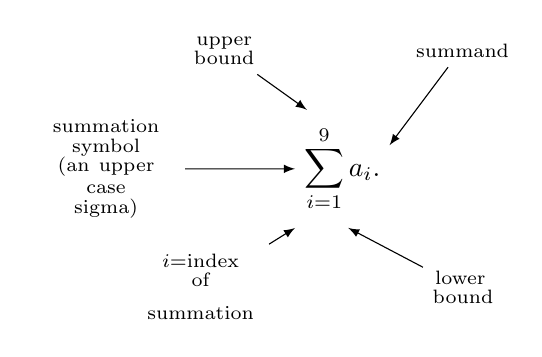
\begin{tikzpicture}[scale=1.5,>=latex]
%\draw [thin,step=1cm] (0,0) grid  (3,3);
\draw  (1,1) node {$\displaystyle \sum_{i=1}^9 a_i$.};

\draw [{\colorone}] (-.2,0) node [text width=45pt,align=center](a) {\scriptsize \centering $i$=index \\[-5pt] of summation};
\draw [{\colorone},->] (a) -- (.6,.5);

\draw [{\colorone}] (2,0) node [text width=20pt,align=center] (b) {\scriptsize \centering lower\\[-5pt] bound};
\draw [{\colorone},->] (b) -- (1.05,.5);

\draw [{\colorone}] (0,2) node [text width=32pt,align=center] (c) {\scriptsize \centering upper\\[-5pt] bound};
\draw [{\colorone},->] (c) -- (.7,1.5);

\draw [{\colorone}] (2,2) node [text width=32pt,align=center] (d) {\scriptsize \centering summand};
\draw [{\colorone},->] (d) -- (1.4,1.2);

\draw [{\colorone}] (-1,1) node [text width=50pt,align=center] (e) {\scriptsize \centering summation \\[-1pt] symbol \\[-1pt] (an upper case\\[-5pt] sigma)};
\draw [{\colorone},->] (e) -- (.6,1);
\end{tikzpicture}
\caption{Understanding sigma notation.}\label{fig:rie_notation}
\end{center}

The upper case sigma represents the term ``sum.'' The index of summation in this example is $i$; any symbol can be used. By convention, the index takes on only the integer values between (and including) the lower and upper bounds. 

Let's practice using this notation.\\

\begin{example}{Using sigma notation}{ex_rie3}{
Let the numbers $\{a_i\}$ be defined as $a_i = 2i-1$ for integers $i$, where $i\geq 1$. So $a_1 = 1$, $a_2 = 3$, $a_3 = 5$, etc. (The output is the positive odd integers). Evaluate the following summations:
$$ 1.\ \sum_{i=1}^6 a_i \qquad\qquad\qquad 2.\ \sum_{i=3}^7 (3a_i-4)\qquad\qquad \qquad 3.\ \sum_{i=1}^4 (a_i)^2$$
}
\end{example}
\begin{solution}
{\begin{enumerate}
		\item		\noindent\vskip-45pt%\begin{minipage}[t]{\linewidth}
						\begin{align*}
						\sum_{i=1}^6 a_i &= a_1+a_2+a_3+a_4+a_5+a_6\\
														&=	1+3+5+7+9+11 \\
														&=	36.
					\end{align*}
%					\end{minipage}
		\item	Note the starting value is different than 1:
					\begin{align*}
					\sum_{i=3}^7 a_i &= (3a_3-4)+(3a_4-4)+(3a_5-4)+(3a_6-4)+(3a_7-4) \\
														&= 11+17+23+29+35 \\
														&= 115.
					\end{align*}
		\item		\noindent\vskip-45pt%\begin{minipage}[t]{\linewidth}
						\begin{align*}
						\sum_{i=1}^4 (a_i)^2 &=	(a_1)^2+(a_2)^2+(a_3)^2+(a_4)^2\\
																&=	1^2+3^2+5^2+7^2 \\
																&=	84
						\end{align*}
\end{enumerate}												
}
\end{solution}


It might seem odd to stress a new, concise way of writing summations only to write each term out as we add them up. It is. The following theorem gives some of the properties of summations that allow us to work with them without writing individual terms. The first three properties are typically referred to as the \textit{linearity properties}. Examples will follow.

\begin{theorem}{Properties of Summations}{summation}
{\noindent\begin{minipage}[t]{200pt}\index{summation!properties}
\begin{enumerate}
		\item		$\ds \sum_{i=1}^n c = c\cdot n$, where $c$ is a constant.
		\item		$\ds \sum_{i=m}^n (a_i\pm b_i) = \sum_{i=m}^n a_i \pm \sum_{i=m}^n b_i$
		\item		$\ds \sum_{i=m}^n c\cdot a_i = c\cdot\sum_{i=m}^n a_i$
		\item		$\ds \sum_{i=m}^j a_i + \sum_{i=j+1}^n  a_i = \sum_{i=m}^n a_i$
%		\item		$\ds \sum_{i=1}^n i = \frac{n(n+1)}2$
%		\item		$\ds \sum_{i=1}^n i^2 = \frac{n(n+1)(2n+1)}6$
%		\item		$\ds \sum_{i=1}^n i^3 = \left(\frac{n(n+1)}2\right)^2$
	\end{enumerate}
\end{minipage}
\begin{minipage}[t]{200pt}
\begin{enumerate}\addtocounter{enumi}{4}
%		\item		$\ds \sum_{i=1}^n c = c\cdot n$, where $c$ is a constant.
%		\item		$\ds \sum_{i=m}^n (a_i\pm b_i) = \sum_{i=m}^n a_i \pm \sum_{i=m}^n b_i$
%		\item		$\ds \sum_{i=1}^n c\cdot a_i = c\cdot\sum_{i=1}^n a_i$
%		\item		$\ds \sum_{i=m}^j a_i + \sum_{i=j+1}^n  a_i = \sum_{i=m}^n a_i$
		\item		$\ds \sum_{i=1}^n i = \frac{n(n+1)}2$
		\item		$\ds \sum_{i=1}^n i^2 = \frac{n(n+1)(2n+1)}6$
		\item		$\ds \sum_{i=1}^n i^3 = \left(\frac{n(n+1)}2\right)^2$
	\end{enumerate}
\end{minipage}
}

\end{theorem}

\begin{example}{Evaluating summations using Theorem \ref{thm:summation}}{ex_rie4}
{Revisit Example \ref{exa:ex_rie3} and, using Theorem \ref{thm:summation}, evaluate $$\sum_{i=1}^6 a_i = \sum_{i=1}^6 (2i-1).$$
}
\end{example}
\begin{solution}
{\begin{align*}
		\sum_{i=1}^6 (2i-1) & = \sum_{i=1}^6 2i - \sum_{i=1}^6 (1)\\
												&=	\left(2\sum_{i=1}^6 i \right)- 6 \\
												&= 2\frac{6(6+1)}{2} - 6 \\
												&= 42-6 = 36
 \end{align*}
 We obtained the same answer without writing out all six terms. When dealing with small sizes of $n$, it may be faster to write the terms out by hand. However, Theorem \ref{thm:summation} is incredibly important when dealing with large sums as we'll soon see.
 }
 \end{solution}


\subsection{Approximating the Area of a Plane Region}
As we have observed above, if $ f(t) $ is a positive velocity function, then the area under the graph of $ f(x) $ over the interval $ [t_1,t_2] $ is the distance travelled over the same time interval.  Note that if $ f(t) $ is allowed to be negative, then the area provides the displacement over the interval.\\  




% left hand sums
%\begin{tikzpicture}[/pgf/declare function={f=4/x;}]
%\begin{axis}[
%        xmin=0,xmax=9,ymin=0,ymax=4,
%    domain=0:10,
%    samples=100,
%    axis lines=middle
%]
%\addplot [thick, red] {f};
%\addplot [
%    black!80,fill=green,opacity=.3,
%    left segments=7,
%    left=1:8
%] {f};
%\end{axis}
%\end{tikzpicture}





For the rest of this section, we assume that $f(x)$ is {\bf{continuous and positive}}, so that the graph lies above the $x$-axis. Our goal is to compute the area ``under the graph", that is, the area between the graph and the $x$-axis.  As a first step, we approximate the area using rectangles.\\

There are three common ways to determine the height of these rectangles: the \textbf{Right Hand Rule} (LHR), the \textbf{Left Hand Rule} (RHR), and the \textbf{Midpoint Rule} (MPR). The \textbf{Riight Hand Rule} says to evaluate the function at the right--hand endpoint of the subinterval and make the rectangle that height. 

The \textbf{Left Hand Rule} says the opposite: on each subinterval, evaluate the function at the left endpoint and make the rectangle that height. 

The \textbf{Midpoint Rule} says that on each subinterval, evaluate the function at the midpoint and make the rectangle that height. 


%Suppose we wish to find the area under $y = x^2$ between $x = 0$ and $x = 1$. 
%
%\begin{tikzpicture}[/pgf/declare function={f=x^2;}]
%\begin{axis}[
%        xmin=0,xmax=1.1,ymin=0,ymax=2,
%    domain=0:1.1,
%    samples=100,
%    axis lines=middle
%]
%\addplot [thick, red, ,name path=A] {f};
% \addplot [draw=none,name path=B] {0};     % “fictional” curve
%  \addplot [green] fill between[of=A and B,soft clip={domain=0:1}]; % filling
%\end{axis}
%\end{tikzpicture}
%
%
%
%
%We can first approximate the area using the RHR. Divide $[0,1]$ into three strips of width $\frac{1}{3}$, and draw rectangles in those strips, the heights of which are the same as the height of the function at the right end of that strip. Four strips gives a better approximation, and five is even better...\\
%\begin{figure}
%% right hand sums
%\begin{tikzpicture}[scale=.75,/pgf/declare function={f=x^2;}]
%\begin{axis}[
%        xmin=0,xmax=1.1,ymin=0,ymax=1.5,
%    domain=0:1.1,
%    samples=100,
%    axis lines=middle,
%     xticklabel style={/pgf/number format/frac, /pgf/number format/frac shift=2},
%     xtick parsed={0, 1/3, 2/3, 1}
%]
%\addplot [
%    black!80,fill=green,opacity=.3,
%    right segments=3,
%    right=0:1,
%] {f};
%\addplot [thick, red] {f};
%\end{axis}
%\end{tikzpicture}
%\begin{tikzpicture}[scale=.75,/pgf/declare function={f=x^2;}]
%\begin{axis}[
%        xmin=0,xmax=1.1,ymin=0,ymax=1.5,
%    domain=0:1.1,
%    samples=100,
%    axis lines=middle,
%     xticklabel style={/pgf/number format/frac, /pgf/number format/frac shift=2},
%     xtick parsed={0, 1/4, 1/2, 3/4, 1}
%]
%\addplot [
%    black!80,fill=green,opacity=.3,
%    right segments=4,
%    right=0:1,
%] {f};
%\addplot [thick, red] {f};
%\end{axis}
%\end{tikzpicture}
%\begin{tikzpicture}[scale=.75,/pgf/declare function={f=x^2;}]
%\begin{axis}[
%        xmin=0,xmax=1.1,ymin=0,ymax=1.5,
%    domain=0:1.1,
%    samples=100,
%    axis lines=middle,
%     xticklabel style={/pgf/number format/frac, /pgf/number format/frac shift=2},
%     xtick parsed={0, 1/5, 2/5, 3/5, 4/5, 1}
%]
%\addplot [
%    black!80,fill=green,opacity=.3,
%    right segments=5,
%    right=0:1,
%] {f};
%\addplot [thick, red] {f};
%\end{axis}
%\end{tikzpicture}
%
%\caption{Approximating the area under $ f(x)=x^2 $ using the RHR, $ n=3, 4,$ and $ 5 $ (right-hand) rectangles, respectively. \label{fig:ApproxAreaRHR1}}
%\end{figure}
%
%
%
%If we use more and more rectangles we get better and better approximations.
%
%\begin{figure}
%\begin{tikzpicture}[scale=.75,/pgf/declare function={f=x^2;}]
%\begin{axis}[
%        xmin=0,xmax=1.1,ymin=0,ymax=1.5,
%    domain=0:1.1,
%    samples=100,
%    axis lines=middle,
%     ]
%\addplot [
%    black!80,fill=green,opacity=.3,
%    right segments=10,
%    right=0:1,
%] {f};
%\addplot [thick, red] {f};
%\end{axis}
%\end{tikzpicture}
%\begin{tikzpicture}[scale=.75,/pgf/declare function={f=x^2;}]
%\begin{axis}[
%        xmin=0,xmax=1.1,ymin=0,ymax=1.5,
%    domain=0:1.1,
%    samples=100,
%    axis lines=middle,
%     ]
%\addplot [
%    black!80,fill=green,opacity=.3,
%    right segments=20,
%    right=0:1,
%] {f};
%\addplot [thick, red] {f};
%\end{axis}
%\end{tikzpicture}
%\begin{tikzpicture}[scale=.75,/pgf/declare function={f=x^2;}]
%\begin{axis}[
%        xmin=0,xmax=1.1,ymin=0,ymax=1.5,
%    domain=0:1.1,
%    samples=100,
%    axis lines=middle,
%     ]
%\addplot [
%    black!80,fill=green,opacity=.3,
%    right segments=40,
%    right=0:1,
%] {f};
%\addplot [thick, red] {f};
%\end{axis}
%\end{tikzpicture}
%
%\caption{Approximating the area under $ f(x)=x^2 $ using the RHR, $ n=10, 20,$ and $ 40 $ (right-hand) rectangles, respectively. \label{fig:ApproxAreaRHR2}}
%\end{figure}
%
%
% Alternatively, we could use the LHR to determine the heights of the rectangles.
%
%\begin{figure}
%\begin{tikzpicture}[scale=.7,/pgf/declare function={f=x^2;}]
%\begin{axis}[
%        xmin=0,xmax=1.2,ymin=0,ymax=2,
%    domain=0:1.1,
%    samples=100,
%    axis lines=middle,
%    xticklabel style={/pgf/number format/frac, /pgf/number format/frac shift=2},
%         xtick parsed={0, 1/3, 2/3, 1}
%]
%\addplot [
%    black!80,fill=green, opacity=.2,
%    left segments=3,
%    left=0:1
%] {f};
%\addplot [thick, red] {f};
%\end{axis}
%\end{tikzpicture}
%\begin{tikzpicture}[scale=.7,/pgf/declare function={f=x^2;}]
%\begin{axis}[
%        xmin=0,xmax=1.2,ymin=0,ymax=2,
%    domain=0:1.1,
%    samples=100,
%    axis lines=middle,
%    xticklabel style={/pgf/number format/frac, /pgf/number format/frac shift=2},
%         xtick parsed={0, 1/4, 1/2, 3/4,1}
%]
%\addplot [
%    black!80,fill=green, opacity=.2,
%    left segments=4,
%    left=0:1
%] {f};
%\addplot [thick, red] {f};
%\end{axis}
%\end{tikzpicture}
%\begin{tikzpicture}[scale=.7,/pgf/declare function={f=x^2;}]
%\begin{axis}[
%        xmin=0,xmax=1.2,ymin=0,ymax=2,
%    domain=0:1.1,
%    samples=100,
%    axis lines=middle,
%    xticklabel style={/pgf/number format/frac, /pgf/number format/frac shift=2},
%         xtick parsed={0, 1/5, 2/5, 3/5,4/5,1}
%]
%\addplot [
%    black!80,fill=green, opacity=.2,
%    left segments=5,
%    left=0:1
%] {f};
%\addplot [thick, red] {f};
%\end{axis}
%\end{tikzpicture}
%\caption{Approximating the area under $ f(x)=x^2 $ using the LHR, $ n=3, 4,$ and $ 5 $ (left-hand) rectangles, respectively. \label{fig:ApproxAreaLHR}}
%\end{figure}
%
%
%We could also use the midpoint rule (MPR).
%
%\begin{figure}
%% mid point
%\begin{tikzpicture}[/pgf/declare function={f=x^2;}]
%\begin{axis}[
%        xmin=0,xmax=1.2,ymin=0,ymax=2,
%    domain=0:1.1,
%    samples=100,
%    axis lines=middle
%]
%\addplot [
%    black!80,fill=green,opacity=.3,
%    midpoint segments=3,
%    midpoint=0:1,
%] {f};
%\addplot [thick,red] {f};
%\end{axis}
%\end{tikzpicture}
%% mid point
%\begin{tikzpicture}[/pgf/declare function={f=x^2;}]
%\begin{axis}[
%        xmin=0,xmax=1.2,ymin=0,ymax=2,
%    domain=0:1.1,
%    samples=100,
%    axis lines=middle
%]
%\addplot [
%    black!80,fill=green,opacity=.3,
%    midpoint segments=4,
%    midpoint=0:1,
%] {f};
%\addplot [thick,red] {f};
%\end{axis}
%\end{tikzpicture}
%% mid point
%\begin{tikzpicture}[/pgf/declare function={f=x^2;}]
%\begin{axis}[
%        xmin=0,xmax=1.2,ymin=0,ymax=2,
%    domain=0:1.1,
%    samples=100,
%    axis lines=middle
%]
%\addplot [
%    black!80,fill=green,opacity=.3,
%    midpoint segments=5,
%    midpoint=0:1,
%] {f};
%\addplot [thick,red] {f};
%\end{axis}
%\end{tikzpicture}
%
%
%\caption{Approximating the area under $ f(x)=x^2 $ using the MPR, $ n=3, 4,$ and $ 5 $ (mid-point) rectangles, respectively. \label{fig:ApproxAreaMP}}
%\end{figure}


\begin{example}{Using the Left Hand, Right Hand and Midpoint Rules}{ex_rie2}
 
Approximate the value of $\int_0^4 (4x-x^2)\ dx$ using the Left Hand Rule, the Right Hand Rule, and the Midpoint Rule, using 4 equally spaced subintervals.
\end{example}

\begin{solution} 
 We break the interval $[0,4]$ into four subintervals. In Figure \ref{fig:rie2a} we see 4 rectangles drawn on $f(x) = 4x-x^2$ using the Left Hand Rule. 

\begin{minipage}[t]{\linewidth}
%\begin{figure}
\begin{center}
\begin{tikzpicture}[/pgf/declare function={f=(4*x-x^2);}]
\begin{axis}[
        xmin=0,xmax=4.1,ymin=0,ymax=4.5,
    domain=0:4,
    samples=100,
    axis lines=middle,
   % xticklabel style={/pgf/number format/frac, /pgf/number format/frac shift=2},
   %      xtick parsed={0, 1, 2, 3, 4}
]
\addplot [
    black!80,fill=green, opacity=.2,
    left segments=4,
    left=0:4,
] {f};
\addplot [thick, red] {f};
\end{axis}
\end{tikzpicture}
\caption{Approximating the area under $f(x)= 4x-x^2$ on $ [0,4] $ using the Left Hand Rule \label{fig:rie2a}}
\end{center}
\end{minipage}
%\end{figure}

\noindent Note how in the first subinterval, $[0,1]$, the rectangle has height $f(0)=0$. We add up the areas of each rectangle (height$\times$ width) for our Left Hand Rule approximation:
	\begin{align*} f(0)\cdot 1 + f(1)\cdot 1+ f(2)\cdot 1+f(3)\cdot 1 &=\\
	0+3+4+3&= 10.
	\end{align*}
	
Figure \ref{fig:rie2b} shows 4 rectangles drawn under $f$ using the Right Hand Rule; note how the $[3,4]$ subinterval has a rectangle of height 0. 

\begin{minipage}[t]{\linewidth}
\begin{center}
\begin{tikzpicture}[/pgf/declare function={f=4*x-x^2;}]
\begin{axis}[
        xmin=0,xmax=4.1,ymin=0,ymax=4.5,
            domain=0:4,
            samples=100,
            axis lines=middle,
         %   xticklabel style={/pgf/number format/frac, /pgf/number format/frac shift=2},
         %        xtick parsed={0, 1, 2, 3, 4}
]
\addplot [
    black!80,fill=green, opacity=.2,
    right segments=4,
    right=0:4
] {f};
\addplot [thick, red] {f};
\end{axis}
\end{tikzpicture}
\caption{Approximating the area under $f(x)= 4x-x^2$ on $ [0,4] $ using the Right Hand Rule \label{fig:rie2b}}
\end{center}
\end{minipage}

\noindent In this example, these rectangle seem to be the mirror image of those found in Figure \ref{fig:rie2a}. (This is because of the symmetry of our shaded region.) Our approximation gives the same answer as before, though calculated a different way:
	\begin{align*} f(1)\cdot 1 + f(2)\cdot 1+ f(3)\cdot 1+f(4)\cdot 1 &=\\
	3+4+3+0&= 10.
	\end{align*}

Figure \ref{fig:rie2c} shows 4 rectangles drawn under $f$ using the Midpoint Rule.

\begin{minipage}[t]{\linewidth}
\begin{center}
\begin{tikzpicture}[/pgf/declare function={f=4*x-x^2;}]
\begin{axis}[
       xmin=0,xmax=4.1,ymin=0,ymax=4.5,
           domain=0:4,
           samples=100,
           axis lines=middle,
       %    xticklabel style={/pgf/number format/frac, /pgf/number format/frac shift=2},
      %          xtick parsed={0, 1, 2, 3, 4}
]
\addplot [
    black!80,fill=green, opacity=.2,
    midpoint segments=4,
    midpoint=0:4
] {f};
\addplot [thick, red] {f};
\end{axis}
\end{tikzpicture}
\caption{Approximating the area under $f(x)= 4x-x^2$ on $ [0,4] $ using the Midpoint Rule \label{fig:rie2c}}
\end{center}
\end{minipage}

\noindent This gives an approximation of 
\begin{align*} f(0.5)\cdot 1 + f(1.5)\cdot 1+ f(2.5)\cdot 1+f(3.5)\cdot 1 &=\\
	1.75+3.75+3.75+1.75&= 11.
	\end{align*}
Our three methods provide two approximations of the area under $f(x)=4x-x^2 $ on $ [0.4] $: 10 and 11.
\end{solution}







% % % % % % % % % % % % % % % % % % % % % % % % %




\subsection{Riemann Sums}


For now, we continue to focus on determining an accurate estimate of area through the use of a sum of the areas of rectangles, doing so in the setting where $f(x) \ge 0$ on $[a,b]$.  Throughout, unless otherwise indicated, we also assume that $f$ is continuous on $[a,b]$.

The first choice we make in any such approximation is the number of rectangles.  
\begin{figure}[h]
\begin{center}
\includegraphics{figures/4_2_Interval}
\caption{Subdividing the interval $[a,b]$ into $n$ subintervals of equal length $\triangle x$.} \label{F:4.2.Interval}
\end{center}
\end{figure}
If we say that the total number of rectangles is $n$, and we desire $n$ rectangles of equal width to subdivide the interval $[a,b]$, then each rectangle must have width $\triangle x = \frac{b-a}{n}$. We observe further that $x_1 = x_0 + \triangle x$, $x_2 = x_0 + 2 \triangle x$, and thus in general $x_{i} = a + i\triangle x,$ as pictured in Figure~\ref{F:4.2.Interval}.

We use each subinterval $[x_i, x_{i+1}]$ as the base of a rectangle, and next must choose how to decide the height of the rectangle that will be used to approximate the area under $y = f(x)$ on the subinterval.  The three standard choices are the left endpoint, right endpoint, or the midpoint of each.  These are precisely the options encountered in the previous section.  We next explore how these choices can be reflected in sigma notation.

If we now consider an arbitrary positive function $f$ on $[a,b]$ with the interval subdivided as shown in Figure~\ref{F:4.2.Interval}, and choose to use left endpoints, then on each interval of the form $[x_{i}, x_{i+1}]$, the area of the rectangle formed is given by
$$A_{i+1} = f(x_i) \cdot \triangle x,$$
as seen in Figure~\ref{F:4.2.LeftSum}.
\begin{figure}[h]
\begin{center}
\includegraphics{figures/4_2_LeftSum}
\caption{Subdividing the interval $[a,b]$ into $n$ subintervals of equal length $\triangle x$ and approximating the area under $y = f(x)$ over $[a,b]$ using left rectangles.} \label{F:4.2.LeftSum}
\end{center}
\end{figure}
If we let $L_n$ denote the sum of the areas of rectangles whose heights are given by the function value at each respective left endpoint, then we see that
\begin{eqnarray*}
L_n & = & A_1 + A_2 + \cdots + A_{i+1} + \cdots + A_n \\
	& = & f(x_0) \cdot \triangle x + f(x_1) \cdot \triangle x + \cdots + f(x_i) \cdot \triangle x + \cdots + f(x_{n-1}) \cdot \triangle x.
\end{eqnarray*}
In the more compact sigma notation, we have 
$$L_n = \sum_{i = 0}^{n-1} f(x_i) \triangle x.$$
Note particularly that since the index of summation begins at $0$ and ends at $n-1$, there are indeed $n$ terms in this sum.  We call $L_n$ the \emph{left Riemann sum} \index{Riemann sum} \index{Riemann sum!left} for the function $f$ on the interval $[a,b]$.

There are now two fundamental issues to explore:  the number of rectangles we choose to use and the selection of the pattern by which we identify the height of each rectangle.  It is best to explore these choices dynamically, and the applet\footnote{Marc Renault, Geogebra Calculus Applets.} found at \href{http://gvsu.edu/s/a9}{\texttt{http://gvsu.edu/s/a9}} is a particularly useful one.  There we see
\begin{figure}[h]
\begin{center}
\scalebox{0.35}{\includegraphics{figures/4_2_RenaultAppletRS.pdf}}
\caption{A snapshot of the applet found at \href{http://gvsu.edu/s/a9}{\texttt{http://gvsu.edu/s/a9}}.} \label{F:4.2.RenaultAppletRS}
\end{center}
\end{figure}
the image shown in Figure~\ref{F:4.2.RenaultAppletRS}, but with the opportunity to adjust the slider bars for the left endpoint and the number of subintervals.  By moving the sliders, we can see how the heights of the rectangles change as we consider left endpoints, midpoints, and right endpoints, as well as the impact that a larger number of narrower rectangles has on the approximation of the exact area bounded by the function and the horizontal axis.  

To see how the Riemann sums for right endpoints and midpoints are constructed, we consider Figure~\ref{F:4.2.RightMidSum}.
\begin{figure}[h]
\begin{center}
\includegraphics{figures/4_2_RightMidSum}
\caption{Riemann sums using right endpoints and midpoints.} \label{F:4.2.RightMidSum}
\end{center}
\end{figure}
For the sum with right endpoints, we see that the area of the rectangle on an arbitrary interval $[x_i, x_{i+1}]$ is given by
$$B_{i+1} = f(x_{i+1}) \cdot \triangle x,$$
so that the sum of all such areas of rectangles is given by
\begin{eqnarray*}
R_n & = & B_1 + B_2 + \cdots + B_{i+1} + \cdots + B_n \\
	& = &  f(x_1) \cdot \triangle x + f(x_2) \cdot \triangle x + \cdots + f(x_{i+1}) \cdot \triangle x + \cdots + f(x_{n}) \cdot \triangle x \\ 
	& = & \sum_{i=1}^{n} f(x_i) \triangle x.
\end{eqnarray*}
We call $R_n$ the \emph{right Riemann sum} \index{Riemann sum!right} for the function $f$ on the interval $[a,b]$.  For the sum that uses midpoints, we introduce the notation
$$\overline{x}_{i+1} = \frac{x_{i} + x_{i+1}}{2}$$
so that $\overline{x}_{i+1}$ is the midpoint of the interval $[x_i, x_{i+1}]$.  For instance, for the rectangle with area $C_1$ in Figure~\ref{F:4.2.RightMidSum}, we now have
$$C_1 = f(\overline{x}_1) \cdot \triangle x.$$
Hence, the sum of all the areas of rectangles that use midpoints is 
\begin{eqnarray*}
M_n & = & C_1 + C_2 + \cdots + C_{i+1} + \cdots + C_n \\
	& = &  f(\overline{x_1}) \cdot \triangle x + f(\overline{x_2}) \cdot \triangle x + \cdots + f(\overline{x}_{i+1}) \cdot \triangle x + \cdots + f(\overline{x}_{n}) \cdot \triangle x \\ 
	& = & \sum_{i=1}^{n} f(\overline{x}_i) \triangle x,
\end{eqnarray*}
and we say that $M_n$ is the \emph{middle (or midpoint) Riemann sum} \index{Riemann sum!middle} for $f$ on $[a,b]$.

When $f(x) \ge 0$ on $[a,b]$, each of the Riemann sums $L_n$, $R_n$, and $M_n$ provides an estimate of the area under the curve $y = f(x)$ over the interval $[a,b]$. As $ n $ increases, each of the approximations get better and better:

\begin{figure}
\begin{subfigure}{.33\textwidth}
  \begin{tikzpicture}[scale=.75,/pgf/declare function={f=x^2;}]
  \begin{axis}[
          xmin=0,xmax=1.1,ymin=0,ymax=1.5,
      domain=0:1.1,
      samples=10,
      axis lines=middle,
       ]
  \addplot [
      black!80,fill=green,opacity=.3,
      right segments=4,
      right=0:1,
  ] {f};
  \addplot [thick, red] {f};
  \end{axis}
  \end{tikzpicture}
  \caption{}
  \label{fig:approx_area1}
\end{subfigure}%
\begin{subfigure}{.33\textwidth}
  \begin{tikzpicture}[scale=.75,/pgf/declare function={f=x^2;}]
  \begin{axis}[
          xmin=0,xmax=1.1,ymin=0,ymax=1.5,
      domain=0:1.1,
      samples=10,
      axis lines=middle,
       ]
  \addplot [
      black!80,fill=green,opacity=.3,
      right segments=10,
      right=0:1,
  ] {f};
  \addplot [thick, red] {f};
  \end{axis}
  \end{tikzpicture}
  \caption{}
  \label{fig:approx_area2}
\end{subfigure}
\begin{subfigure}{.33\textwidth}
  \begin{tikzpicture}[scale=.75,/pgf/declare function={f=x^2;}]
  \begin{axis}[
          xmin=0,xmax=1.1,ymin=0,ymax=1.5,
      domain=0:1.1,
      samples=10,
      axis lines=middle,
       ]
  \addplot [
      black!80,fill=green,opacity=.3,
      right segments=40,
      right=0:1,
  ] {f};
  \addplot [thick, red] {f};
  \end{axis}
  \end{tikzpicture}
  \caption{}
  \label{fig:approx_area3}
\end{subfigure}
\caption{The approximations get better and better as the number of strips ($ n $) increases. \label{fig:subst12}}
\label{fig:test}
\end{figure}



The following example lets us practice using the Right Hand Rule and the summation formulas introduced in Theorem \ref{thm:summation}.\\

\begin{example}{Approximating definite integrals using sums}{ex_rie7}
{
Approximate the area $ A $ under $f(x) = 4x-x^2 \ dx$ on $ [0,4] $ using the Right Hand Rule with 16 and 1000 equally spaced intervals.
}
\end{example}

\begin{solution}
{Using 16 equally spaced intervals and the Right Hand Rule, we can approximate the area as 
$$\sum_{i=1}^{16}f(x_{i+1})\Delta x.$$
We have $\Delta x = 4/16 = 0.25$. Since $x_i = 0+(i-1)\Delta x$, we have 
\begin{align*}
x_{i+1} &= 0 + \big((i+1)-1\big)\Delta x \\
				&=	i\Delta x
\end{align*}
%In our examples using the Right Hand Rule is simpler notationally as $f(x_{i+1}) = f(i\Delta x)$. 
This gives:\\
\begin{minipage}{.6\textwidth}

\begin{align}
\text{ Area } = A  &\approx \sum_{i=1}^{16} f(x_{i+1})\Delta x \notag\\
											&= \sum_{i=1}^{16} f(i\Delta x) \Delta x\notag\\
									&= \sum_{i=1}^{16} \big(4i\Delta x - (i\Delta x)^2\big)\Delta x\notag\\
									&= \sum_{i=1}^{16} (4i\Delta x^2 - i^2\Delta x^3)\notag\\		
									&= (4\Delta x^2)\sum_{i=1}^{16} i - \Delta x^3 \sum_{i=1}^{16} i^2 \label{eq:rie7}\\
									&= (4\Delta x^2)\frac{16\cdot 17}{2} - \Delta x^3 \frac{16(17)(33)}6 \notag\\
									&=	4\cdot 0.25^2\cdot 136-0.25^3\cdot 1496\notag\\
									&=10.625\notag
\end{align}
\end{minipage}
\begin{minipage}{.35\textwidth}
\begin{center}
\begin{tikzpicture}[scale=.75,/pgf/declare function={f=(4*x-x^2);}]
  \begin{axis}[
          xmin=0,xmax=4.1,ymin=0,ymax=4.1,
      domain=0:4,
      samples=10,
      axis lines=middle,
       ]
  \addplot [
      black!80,fill=green,opacity=.3,
      right segments=16,
      right=0:4,
  ] {f};
  \addplot [thick, red] {f};
	  \end{axis}
  \end{tikzpicture}
  \caption{ \label{fig:rie7} %Approximating with the Right Hand Rule and 16 evenly spaced subintervals.
  }
\end{center}
\end{minipage}

We were able to sum up the areas of 16 rectangles with very little computation. In Figure \ref{fig:rie7} the function and the 16 rectangles are graphed. 

%\begin{minipage}[c]{.5\textwidth}
%\centering
%\begin{tikzpicture}[scale=.75,/pgf/declare function={f=(4*x-x^2);}]
%  \begin{axis}[
%          xmin=0,xmax=4.1,ymin=0,ymax=4.1,
%      domain=0:4,
%      samples=10,
%      axis lines=middle,
%       ]
%  \addplot [
%      black!80,fill=green,opacity=.3,
%      right segments=16,
%      right=0:4,
%  ] {f};
%  \addplot [thick, red] {f};
%	  \end{axis}
%  \end{tikzpicture}
%\captionof{figure}{} %{Approximating with the Right Hand Rule and 16 evenly spaced subintervals.}
%\label{fig:rie7}
%\end{minipage}

While some rectangles over--approximate the area, others under--approximate the area (by about the same amount). Thus our approximate area of 10.625 is likely a fairly good approximation. 

Notice  Equation \eqref{eq:rie7}; by changing the 16's to 1,000's (and appropriately changing the value of $\Delta x$), we can use that equation to sum up 1000 rectangles!


We do so here, skipping from the original summand to the equivalent of Equation \eqref{eq:rie7} to save space. Note that $\Delta x = 4/1000 = 0.004$.
\begin{align}
A &\approx \sum_{i=1}^{1000} f(x_{i+1})\Delta x \notag\\
									&= (4\Delta x^2)\sum_{i=1}^{1000} i - \Delta x^3 \sum_{i=1}^{1000} i^2 \notag\\
									&= (4\Delta x^2)\frac{1000\cdot 1001}{2} - \Delta x^3 \frac{1000(1001)(2001)}6 \notag\\
									&=	4\cdot 0.004^2\cdot 500500-0.004^3\cdot 333,833,500\notag\\
									&=10.666656\notag
\end{align}

Using many, many rectangles, we have a likely good approximation of the area. That is, $$A \approx 10.666656.$$
}
\end{solution}


The previous example motivates the following definition.

\begin{definition}{Area}{area}
The area $ A $ of the region that lies under the graph of a continuous nonnegative function $ f $ over the interval $ [a,b] $ is the limit of the sum of the areas of approximating rectangles:
\[
A = \lim_{n\to \infty} R_n = \sum_{i=1}^{n} f(x_i) \Delta x, 
\]
where $ \Delta x = \frac{b-a}{n} $, and $ x_i=a+1\Delta x $.
\end{definition}

\begin{example}{Approximating definite integrals with a formula, using sums}{ex_rie9}
{
Revisit Example \ref{exa:ex_rie7}. Use Definition \ref{def:area} to determine the area under $f(x) = 4x-x^2 \ dx$ on $ [0,4] $ .}
\end{example}

\begin{solution}
We have $\Delta x = \frac{4-0}{n} = 4/n$, and $x_i = 0 + \Delta x(i) = 4i/n$.

We construct the Riemann sum as follows. Be sure to follow each step carefully. If you get stuck, and do not understand how one line proceeds to the next, you may skip to the result and consider how this result is used. You should come back, though, and work through each step for full understanding.
\begin{align*}
		R_n &= \sum_{i=1}^n f(x_{i+1})\Delta x \\
											&= \sum_{i=1}^n f\left(\frac{4i}{n}\right) \Delta x \\
											&=	\sum_{i=1}^n \left[4\frac{4i}n-\left(\frac{4i}n\right)^2\right]\Delta x\\
											&=	\sum_{i=1}^n \left(\frac{16\Delta x}{n}\right)i - \sum_{i=1}^n \left(\frac{16\Delta x}{n^2}\right)i^2 \\
											&=	\left(\frac{16\Delta x}{n}\right)\sum_{i=1}^n i - \left(\frac{16\Delta x}{n^2}\right)\sum_{i=1}^n i^2  \\
											&= \left(\frac{16\Delta x}{n}\right)\cdot \frac{n(n+1)}{2} - \left(\frac{16\Delta x}{n^2}\right)\frac{n(n+1)(2n+1)}{6} \quad \left(\parbox{35pt}{\scriptsize \centering recall $\Delta x = 4/n$}\right)\\
											&=\frac{32(n+1)}{n} - \frac{32(n+1)(2n+1)}{3n^2} \quad \text{\scriptsize (now simplify)} \\
											&= \frac{32}{3}\left(1-\frac{1}{n^2}\right)
\end{align*}
Therefore, we have
\[
A=\lim_{n\to \infty}R_n = \lim_{n\to \infty}\frac{32}{3}\left(1-\frac{1}{n^2}\right)=\frac{32}{3}\left(1-0\right)=\frac{32}{3}
\]
Note that our approximation in Example \ref{exa:ex_rie7} using 16 subintervals was actually quite a good estimate. 
\end{solution}




It can be proved that the limit in Definition \ref{def:area} always exists (as $ f $) is assumed to be continuous). Moreover, we get the same value of we take the limit using left endpoints, or midpoints. 



$$A = \lim_{n \to \infty} R_n = \lim_{n \to \infty} L_n = \lim_{n \to \infty} M_n.$$  


Momentarily, we will discuss the meaning of Riemann sums in the setting when $f$ is sometimes negative.  We also recall that in the context of a nonnegative velocity function $y = v(t)$, the corresponding Riemann sums are approximating the distance traveled on $[a,b]$ by the moving object with velocity function $v$.

There is a more general way to think of Riemann sums, and that is to not restrict the choice of where the function is evaluated to determine the respective rectangle heights.  That is, rather than saying we'll always choose left endpoints, or always choose midpoints, we simply say that a point $x_{i+1}^*$ will be selected at random in the interval $[x_i, x_{i+1}]$ (so that $x_i \le x_{i+1}^* \le x_{i+1}$), which makes the Riemann sum given by 
$$f(x_1^*) \cdot \triangle x + f(x_2^*) \cdot \triangle x + \cdots + f(x_{i+1}^*) \cdot \triangle x + \cdots + f(x_n^*) \cdot \triangle x = \sum_{i=1}^{n} f(x_i^*) \triangle x.$$

Definition \ref{def:area} could also be made using this more general Riemann sum:

\begin{formulabox}[Area: another definition]
$$A = \lim_{n \to \infty} R_n = \lim_{n \to \infty} L_n = \lim_{n \to \infty} M_n = \lim_{n \to \infty} \sum_{i=1}^{n} f(x_i^*) \triangle x.$$  
\end{formulabox}

In general, the \textbf{lower} (resp. \textbf{upper}) \textbf{sums} are formed by choosing the sample points $ x_i^* $ so that $ f(x_i^*) $ is the minimum (resp. maximum) value of on the $ i $th subinterval. In the special case that $ f $ is monotone increasing  (resp. decreasing), the left and right endpoint approximations correspond to the lower and upper (resp. upper and lower) sums.
   

\begin{figure}
\centering
\begin{subfigure}{.45\textwidth}
  \begin{tikzpicture}[scale=.75,/pgf/declare function={f=x^2;}]
  \begin{axis}[
          xmin=0,xmax=1.1,ymin=0,ymax=1.5,
      domain=0:1.1,
      samples=10,
      axis lines=middle,
       ]
  \addplot [
      black!80,fill=green,opacity=.3,
      right segments=5,
      right=0:1,
  ] {f};
  \addplot [
        black!80,fill=blue,opacity=.3,
        left segments=5,
        left=0:1,
    ] {f};
  \addplot [thick, red] {f};
  \end{axis}
  \end{tikzpicture}
  \caption{$ f $ monotone increasing:\\ $ L_n\le \text{ Area } \le R_n $}
  \label{fig:approx_area1}
\end{subfigure}%
\begin{subfigure}{.45\textwidth}
  \begin{tikzpicture}[scale=.75,/pgf/declare function={f=(x-1)^2;}]
  \begin{axis}[
          xmin=0,xmax=1.1,ymin=0,ymax=1.5,
      domain=0:1.1,
      samples=10,
      axis lines=middle,
       ]
  \addplot [
        black!80,fill=blue,opacity=.3,
        left segments=5,
        left=0:1,
    ] {f};
    \addplot [
          black!80,fill=green,opacity=.3,
          right segments=5,
          right=0:1,
      ] {f};
  \addplot [thick, red] {f};
  \end{axis}
  \end{tikzpicture}
  \caption{$ f $ monotone decreasing:\\ $ R_n\le \text{ Area } \le L_n $}
  \label{fig:approx_area1}
\end{subfigure}%
\caption{For monttonic functions lower and upper sums are given by $ L_n $ or $ R_n $.}
\label{fig:test}
\end{figure}


At \href{http://gvsu.edu/s/a9}{\texttt{http://gvsu.edu/s/a9}}, the applet noted earlier and referenced in Figure~\ref{F:4.2.RenaultAppletRS}, by unchecking the ``relative'' box at the top left, and instead checking ``random,'' we can easily explore the effect of using random point locations in subintervals on a given Riemann sum.  In computational practice, we most often use $L_n$, $R_n$, or $M_n$, while the random Riemann sum is useful in theoretical discussions.  


\subsection*{When the function is sometimes negative}

For a Riemann sum such as 
$$L_n = \sum_{i=0}^{n-1} f(x_i) \triangle x,$$
we can of course compute the sum even when $f$ takes on negative values.  We know that when $f$ is positive on $[a,b]$, the corresponding left Riemann sum $L_n$ estimates the area bounded by $f$ and the horizontal axis over the interval.  
\begin{figure}[h]
\begin{center}
\includegraphics{figures/4_2_NegF}
\caption{At left and center, two left Riemann sums for a function $f$ that is sometimes negative; at right, the areas bounded by $f$ on the interval $[a,d]$.} \label{F:4.2.NegF}
\end{center}
\end{figure}
For a function such as the one pictured in Figure~\ref{F:4.2.NegF}, where in the first figure a left Riemann sum is being taken with 12 subintervals over $[a,d]$, we observe that the function is negative on the interval $b \le x \le c$, and so for the four left endpoints that fall in $[b,c]$, the terms $f(x_i) \triangle x$ have negative function values.  This means that those four terms in the Riemann sum produce an estimate of the \emph{opposite} of the area bounded by $y = f(x)$ and the $x$-axis on $[b,c]$.

In Figure~\ref{F:4.2.NegF}, we also see evidence that by increasing the number of rectangles used in a Riemann sum, it appears that the approximation of the area (or the opposite of the area) bounded by a curve appears to improve.  For instance, in the middle graph, we use $ 24 $ left rectangles, and from the shaded areas, it appears that we have decreased the error from the approximation that uses 12.  When we proceed to the next section, we will discuss the natural idea of letting the number of rectangles in the sum increase without bound.  

For now, it is most important for us to observe that, in general, any Riemann sum of a continuous function $f$ on an interval $[a,b]$ approximates the difference between the area that lies above the horizontal axis on $[a,b]$ and under $f$ and the area that lies below the horizontal axis on $[a,b]$ and above $f$.  In the notation of Figure~\ref{F:4.2.NegF}, we may say that
$$L_{24} \approx A_1 - A_2 + A_3,$$
where $L_{24}$ is the left Riemann sum using $ 24 $ subintervals shown in the middle graph, and $A_1$ and $A_3$ are the areas of the regions where $f$ is positive on the interval of interest, while $A_2$ is the area of the region where $f$ is negative.  We will also call the quantity $A_1 - A_2 + A_3$ the \emph{net signed area} \index{net signed area} bounded by $f$ over the interval $[a,d]$, where by the phrase ``signed area'' we indicate that we are attaching a minus sign to the areas of regions that fall below the horizontal axis.

Finally, we recall that in the context where the function $f$ represents the velocity of a moving object, the total sum of the areas bounded by the curve tells us the total distance traveled over the relevant time interval, while the total net signed area bounded by the curve computes the object's change in position on the interval.

%\nin \framebox{\hspace*{3 pt}
%\parbox{6.25 in}{
Summary:
\begin{itemize}
\item A Riemann sum is simply a sum of products of the form $f(x_i^*) \triangle x$ that estimates the area between a positive function and the horizontal axis over a given interval.  If the function is sometimes negative on the interval, the Riemann sum estimates the difference between the areas that lie above the horizontal axis and those that lie below the axis.
\item The three most common types of Riemann sums are left, right, and middle sums, plus we can also work with a more general, random Riemann sum.  The only difference among these sums is the location of the point at which the function is evaluated to determine the height of the rectangle whose area is being computed in the sum.  For a left Riemann sum, we evaluate the function at the left endpoint of each subinterval, while for right and middle sums, we use right endpoints and midpoints, respectively.
\item The left, right, and middle Riemann sums are denoted $L_n$, $R_n$, and $M_n$, with formulas
$$L_n = f(x_0) \triangle x + f(x_1) \triangle x + \cdots + f(x_{n-1}) \triangle x = \sum_{i = 0}^{n-1} f(x_i) \triangle x,$$
$$R_n = f(x_1) \triangle x + f(x_2) \triangle x + \cdots + f(x_{n}) \triangle x = \sum_{i = 1}^{n} f(x_i) \triangle x,$$
$$M_n = f(\overline{x}_1) \triangle x + f(\overline{x}_2) \triangle x + \cdots + f(\overline{x}_{n}) \triangle x = \sum_{i = 1}^{n} f(\overline{x}_i) \triangle x,$$
where $x_0 = a$, $x_i = a + i\triangle x$, and $x_n = b$, using $\triangle x = \frac{b-a}{n}$.  For the midpoint sum, $\overline{x}_{i} = (x_{i-1} + x_i)/2$.
\end{itemize}

\subsection{The Definite Integral}

In the previous examples it appears that as the number of rectangles got larger and larger, the values of $L_n$, $M_n$, and $R_n$ all grew closer and closer to the same value.  It turns out that this occurs for any continuous function on an interval $[a,b]$, and even more generally for a Riemann sum using any point $x_{i+1}^*$ in the interval $[x_i, x_{i+1}]$.  Said differently, as we let $n \to \infty$, it doesn't really matter where we choose to evaluate the function within a given subinterval, because
$$\lim_{n \to \infty} L_n = \lim_{n \to \infty} R_n = \lim_{n \to \infty} M_n = \lim_{n \to \infty} \sum_{i=1}^{n} f(x_i^*) \triangle x.$$  
That these limits always exist (and share the same value) for a continuous\footnote{It turns out that a function need not be continuous in order to have a definite integral.  For our purposes, we assume that the functions we consider are continuous on the interval(s) of interest.  It is straightforward to see that any function that is piecewise continuous on an interval of interest will also have a well-defined definite integral.} function $f$ allows us to make the following definition.
\begin{definition} \label{D:4.3.DefInt}
The \emph{definite integral} of a continuous function $f$ on the interval $[a,b]$, denoted $\ds \int_a^b f(x) \, dx$, is the real number given by
$$\int_a^b f(x) \, dx = \lim_{n \to \infty} \sum_{i=1}^{n} f(x_i^*) \triangle x,$$
where $\triangle x = \frac{b-a}{n}$, $x_i = a + i\triangle x$ (for $i = 0, \ldots, n$), and $x_i^*$ satisfies $x_{i-1} \le x_i^* \le x_i$ (for $i = 1, \ldots, n$).
\end{definition}
We call the values $a$ and $b$ the \emph{lower and upper limits of integration} respectively\index{limits of integration}.  The process of determining the real number $\int_a^b f(x) \, dx$ is called \emph{evaluating the definite integral}.  

\begin{example}{Finding definite integrals with Riemann sums}{ex_rie10}
{
Find  $\ds \int_{-1}^5 x^3\ dx$ using the limit definition of the definite integral..
}
\end{example}

\begin{solution}
{As we may choose $ x_i^* $ freely in Definition \ref{def:D:4.3.DefInt}, we will use the right hand rule, so 
we have $\Delta x = (b-a)/n= \frac{5-(-1)}{n} = 6/n$, and $x_i = a+i\Delta x = (-1) +  i \Delta x$.
The Riemann sum corresponding to the Right Hand Rule is (followed by simplifications):
\begin{align*}
\int_{-1}^5 x^3\ dx 	&\approx \sum_{i=1}^n f(x_{i+1})\Delta x \\
											&= \sum_{i=1}^n f(-1+i\Delta x)\Delta x \\
											&= \sum_{i=1}^n (-1+i\Delta x)^3\Delta x \\
											&= \sum_{i=1}^n \big((i\Delta x)^3 -3(i\Delta x)^2 + 3i\Delta x -1\big)\Delta x \quad \text{\scriptsize (now distribute $\Delta x$)} \\
											&= \sum_{i=1}^n \big(i^3\Delta x^4 - 3i^2\Delta x^3 + 3i\Delta x^2 -\Delta x\big) \quad \text{\scriptsize (now split up summation)}\\
%\end{align*}
%\begin{align*}
											&= \Delta x^4 \sum_{i=1}^ni^3 -3\Delta x^3 \sum_{i=1}^n i^2+ 3\Delta x^2 \sum_{i=1}^n i - \sum_{i=1}^n \Delta x \\
											&= \Delta x^4 \left(\frac{n(n+1)}{2}\right)^2 -3\Delta x^3 \frac{n(n+1)(2n+1)}{6}+ 3\Delta x^2 \frac{n(n+1)}{2} - n\Delta x 
												\intertext{\scriptsize (use $\Delta x = 6/n$)}
											&= \frac{1296}{n^4}\cdot\frac{n^2(n+1)^2}{4} - 3\frac{216}{n^3}\cdot\frac{n(n+1)(2n+1)}{6} + 3\frac{36}{n^2}\frac{n(n+1)}2 -6\\
											&= 324\cdot\left(\frac{n+1}{n}\right)^2-108\cdot\frac{n+1}{n}\cdot\frac{2n+1}{n}+54 \cdot\frac{n+1}{n}-6\\ 
											&= 324\cdot\left(1+\frac{1}{n}\right)^2-108\cdot\left(1+\frac{1}{n}\right)\cdot\left(2+\frac{1}{n}\right)+54 \cdot\left(1+\frac{1}{n}\right)-6\\
%											&\frac{1296}{n^4}\cdot\frac{n^2(n+1)^2}{4} - 3\frac{216}{n^3}\cdot\frac{n(n+1)(2n+1)}{6} + 3\frac{36}{n^2}\frac{n(n+1)}2 -6
%											\intertext{\scriptsize (use $\Delta x = 6/n$)}
%											&= \frac{1296}{n^4}\cdot\frac{n^2(n+1)^2}{4} - 3\frac{216}{n^3}\cdot\frac{n(n+1)(2n+1)}{6} + 3\frac{36}{n^2}\frac{n(n+1)}2 -6
%											\intertext{\scriptsize (now do a sizable amount of algebra to simplify)}
%											&=156 + \frac{378}n + \frac{216}{n^2}
\end{align*}

Now find the exact answer using a limit:
$$\int_{-1}^5 x^3\ dx = \lim_{n\to\infty} \left(324\cdot\left(1+\frac{1}{n}\right)^2-108\cdot\left(1+\frac{1}{n}\right)\cdot\left(2+\frac{1}{n}\right)+54 \cdot\left(1+\frac{1}{n}\right)-6\right) = 156.$$
}
\end{solution}


If we wish to compute the value of a definite integral using the definition, we have to take the limit of a sum.  While this is possible to do in select circumstances, it is also tedious and time-consuming; moreover, computing these limits does not offer much additional insight into the meaning or interpretation of the definite integral.  Instead, in the next section, we will learn the Fundamental Theorem of Calculus, a result that provides a shortcut for evaluating a large class of definite integrals.  This will enable us to determine the exact net signed area bounded by a continuous function and the $x$-axis in many circumstances.

While we will come to understand that there are several different interpretations of the value of the definite integral, for now the most important is that $\int_a^b f(x) \, dx$ measures the net signed area bounded by $y = f(x)$ and the $x$-axis on the interval $[a,b]$. 

\begin{figure}[h]
\begin{center}
\includegraphics{figures/4_3_DefIntInterp}
\caption{A continuous function $f$ on the interval $[a,d]$.} \label{F:4.3.DefIntInterp}
\end{center}
\end{figure}
For example, in the notation of the definite integral, if $f$ is the function pictured in Figure~\ref{F:4.3.DefIntInterp} and $A_1$, $A_2$, and $A_3$ are the exact areas bounded by $f$ and the $x$-axis on the respective intervals $[a,b]$, $[b,c]$, and $[c,d]$, then
$$\int_a^b f(x) \, dx = A_1, \ \int_b^c f(x) \, dx = -A_2, \ \int_c^d f(x) \, dx = A_3,$$
and
$$\int_a^d f(x) \, dx = A_1 - A_2 + A_3.$$


If a given curve produces regions whose areas we can compute exactly through known area formulas, we can thus compute the exact value of the integral.  Let's look at a few more examples.



\begin{example}{Finding definite integrals as signed areas}{ex_disa}
Evaluate the following integrals by interpreting each in terms of signed areas:
\begin{enumerate}
\item $ \ds \int_{0}^{2} \sqrt{4-x^2}\; dx $
\item $ \ds \int_{0}^{3} 2-x\; dx $
\item $ \ds \int_1^4 2x+2\; dx $
\item $ \ds \int_{0}^{3} |2-x|\; dx $
\end{enumerate}
\end{example}

\begin{solution}
\begin{enumerate}
\item Since $ f(x) =  \sqrt{4-x^2}\ge 0 $, the integral corresponds to the area under the curve $ y=f(x) $ between $ x=0 $ and $ x=2. $  Since $ y= \sqrt{4-x^2} \Rightarrow y^2=4-x^2\Rightarrow x^2+y^2=4 $, the region we are interested in is that of a quarter circle with radius $ 2 $. So we have

\begin{minipage}[c]{.3\textwidth}
\begin{tikzpicture}[scale=.6,/pgf/declare function={f=sqrt(4-x^2);}]
\begin{axis}[
        xmin=-0.1,xmax=2.1,ymin=-0.1,ymax=2.1,
    domain=0:2,
    samples=100,
    axis lines=middle
]
\addplot [thick, red, ,name path=A] {f};
 \addplot [draw=none,name path=B] {0};     % “fictional” curve
  \addplot [green] fill between[of = A and B,soft clip={domain=0:2}]; % filling
\end{axis}
\end{tikzpicture}
\end{minipage}
\begin{minipage}[c]{.5\textwidth}
\begin{center}
\[
\int_{0}^{2} \sqrt{4-x^2}\; dx = \frac14 \pi (2)^2=\pi.
\]
\end{center}
\end{minipage}
\item The region between the $ x $-axis and $ y=2-x $ over the interval $ [0,3] $ consists of two triangular regions of areas $ 2 $ and $ \frac12 $. Since the second triangle is below the $ x $-axis, it has a signed area of $ -\frac{1}{2} $. so we have 

\begin{minipage}[c]{.3\textwidth}
\begin{tikzpicture}[scale=.6,/pgf/declare function={f= 2-x;}]
\begin{axis}[
        xmin=-1.1,xmax=3.1,ymin=-1.1,ymax=3.1,
    domain=0:3,
    samples=10,
    axis lines=middle
]
\addplot [thick, red, ,name path=A] {f};
 \addplot [draw=none,name path=B] {0};     % “fictional” curve
  \addplot [green] fill between[of = A and B,soft clip={domain=0:2}]; % filling
  \addplot [red] fill between[of = A and B,soft clip={domain=2:3}]; % filling
\end{axis}
\end{tikzpicture}
\end{minipage}
\begin{minipage}[c]{.5\textwidth}
\begin{center}
\[
\int_{0}^{3} 2-x\; dx = 2-\frac12=\frac32.
\]
\end{center}
\end{minipage}

\item Observe that the region bounded by this function and the $x$-axis is the trapezoid, and by the known formula for the area of a trapezoid, its area is $A = \frac{1}{2}(3+9) \cdot 3 = 18$, so

\begin{minipage}[c]{.3\textwidth}
\begin{tikzpicture}[scale=.6,/pgf/declare function={f=2*x+1;}]
\begin{axis}[
        xmin=-1.1,
        xmax=4.3,
        ymin=-1.1,
        ymax=9.2,
    domain=0:4,
    samples=10,
    axis lines=middle,
    xtick={1,4},
    ytick={3,9},
]
\addplot [thick, red, ,name path=A] {f};
 \addplot [draw=none,name path=B] {0};     % “fictional” curve
  \addplot [green] fill between[of = A and B,soft clip={domain=1:4}]; % filling
  %\addplot [red] fill between[of = A and B,soft clip={domain=2:3}]; % filling
\end{axis}
\end{tikzpicture}
\end{minipage}
\begin{minipage}[c]{.5\textwidth}
\begin{center}
$$\int_1^4 (2x+1) \, dx = 18.$$
\end{center}
\end{minipage}


\item The region between the $ x $-axis and $ y=|2-x| $ over the interval $ [0,3] $ consists of two triangular regions of areas $ 2 $ and $ \frac12 $. Both are above the $ x $-axis, so have a positive signed area, and we have 

\begin{minipage}[c]{.3\textwidth}
\begin{tikzpicture}[scale=.6,/pgf/declare function={f=abs(2-x);}]
\begin{axis}[
        xmin=-1.1,
        xmax=3.1,
        ymin=-1.1,
        ymax=3.1,
      domain=0:3,
      samples=10,
    axis lines=middle,
     %xlabel=$t$,
     % ylabel=$v$,
     % xtick={-4,...,4},
     % ytick={1,...,5},
    ]
\addplot [thick, red, ,name path=A] {f};
 \addplot [draw=none,name path=B] {0};     % “fictional” curve
  \addplot [green] fill between[of = A and B,soft clip={domain=0:2}]; % filling
  \addplot [green] fill between[of = A and B,soft clip={domain=2:3}]; % filling
\end{axis}
\end{tikzpicture}
\end{minipage}
\begin{minipage}[c]{.5\textwidth}
\begin{center}
\[
\int_{0}^{3} 2-x\; dx = 2+\frac12=\frac52.
\]
\end{center}
\end{minipage}


\end{enumerate}
\end{solution}






We can also use definite integrals to express the change in position and distance traveled by a moving object.  In the setting of a velocity function $v$ on an interval $[a,b]$, it follows from our work above and in preceding sections that the change in position, $s(b) - s(a)$, is given by
$$s(b) - s(a) = \int_a^b v(t) \, dt.$$
If the velocity function is nonnegative on $[a,b]$, then $\int_a^b v(t) \,dt$ tells us the distance the object travelled.  When velocity is sometimes negative on $[a,b],$ the areas bounded by the function on intervals where $v$ does not change sign can be found using integrals, and the sum of these values will tell us the distance the object travelled. 

\begin{example}{Understanding motion given velocity}{ex_defint6}
{
Consider the graph of a velocity function of an object moving in a straight line, given in Figure \ref{fig:defint6}, where the numbers in the given regions gives the area of that region.  Find the maximum speed of the object and its maximum displacement from its starting position.
}
\end{example}
\begin{center}
\begin{figure}
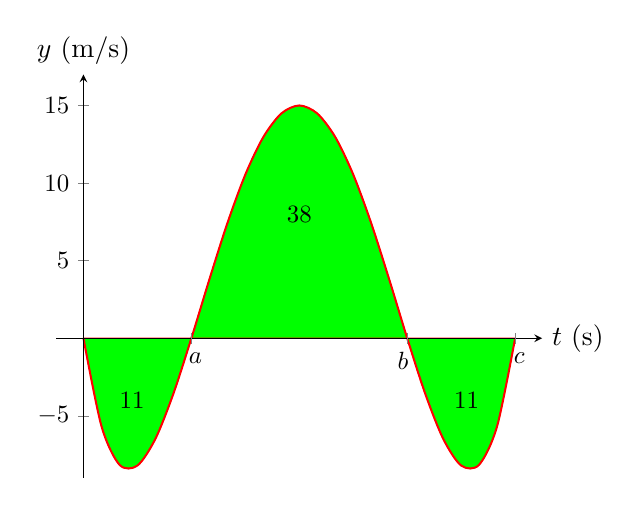
\begin{tikzpicture}[scale=.9]
\begin{axis}[ %width=\marginparwidth+25pt,%
            %tick label style={font=\scriptsize},
            axis y line=middle,
            axis x line=middle,
            name=myplot,
            axis on top,%
			%x=.37\marginparwidth,
			%y=.37\marginparwidth,
			xtick=\empty,% 
			extra x ticks={2,6,8},
			extra x tick labels={$\ a$,$b\ $,$\ c$},
			ytick={-5,5,10,15},
			%minor y tick num=1,%extra y ticks={-5,-3,...,7},%
%			minor x tick num=4,
			ymin=-9,ymax=17,%
			xmin=-.5,xmax=8.5%
]

\addplot [smooth,red,fill={green},area style,domain=0:8] {15/64*x*(x-2)*(x-6)*(x-8)} \closedcycle;
\addplot [smooth,thick,red,domain=0:8] {15/64*x*(x-2)*(x-6)*(x-8)};

\draw (axis cs:.9,-4) node { $11$};
\draw (axis cs:7.1,-4) node { $11$};
\draw (axis cs:4,8) node { $38$};
\end{axis}

\node [right] at (myplot.right of origin) { $t$ (s)};
\node [above] at (myplot.above origin) { $y$ (m/s)};
\end{tikzpicture}
\caption{A graph of a velocity in Example \ref{exa:ex_defint6}.\label{fig:defint6}}
\end{figure}
\end{center}

\begin{solution}
Since the graph gives velocity, finding the maximum speed is simple: it looks to be $ 15 $m/s.

At time $t=0$, the displacement is $ 0 $; the object is at its starting position. At time $t=a$, the object has moved backward $ 11 $ meters. Between times $t=a$ and $t=b$, the object moves forward $ 38 $ meters, bringing it into a position $ 27 $ meters forward of its starting position. From $t=b$ to $t=c$ the object is moving backwards again, hence its total displacement is $ 27 $ meters from its starting position.
\[
\text{Total Displacement} = \int_0^c v(t)\;dt = -11+38-11=16m.
\]
\[
\text{Maximum Displacement} = \int_0^b v(t)\;dt = -11+38=27m.
\]
\end{solution}













\subsection*{Some properties of the definite integral}

With the perspective that the definite integral of a function $f$ over an interval $[a,b]$ measures the net signed area bounded by $f$ and the $x$-axis over the interval, we naturally arrive at several different standard properties of the definite integral.  In addition, it is helpful to remember that the definite integral is defined in terms of Riemann sums that fundamentally consist of the areas of rectangles.

If we consider the definite integral $\int_a^a f(x) \, dx$ for any real number $a$, it is evident that no area is being bounded because the interval begins and ends with the same point.  Hence, 

\vspace*{5pt}
\noindent \framebox{\hspace*{3 pt}
\parbox{6.25 in}{
If $f$ is a continuous function and $a$ is a real number, then $\ds \int_a^a f(x) \,dx = 0.$
} \hspace*{3 pt}}
\vspace*{1pt}
 

Next, we consider the results of subdividing a given interval. In Figure~\ref{F:4.3.AdditiveProp}, we see that
$$\int_a^b f(x) \, dx = A_1, \ \int_b^c f(x) \, dx = A_2, \ \mbox{and} \ \int_a^c f(x) \, dx = A_1 + A_2,$$ 
which is indicative of the following general rule.
  
\begin{figure}[h]
\begin{center}
%\includegraphics{figures/4_3_AdditiveProp}
\begin{tikzpicture}[/pgf/declare function={f=-x^3+5*(x^2)-3*x-3;}]
  \begin{axis}[
    axis y line = left,
    axis x line = bottom,
    xtick       = {-1.2,2,4.2},
    xticklabels = {$a$,$b$,$c$},
     ytick       = {},
    yticklabels = {},
    samples     = 160,
    domain      = -1.2:4.2,
    xmin = -2, xmax = 5,
    ymin = -5, ymax = 10,
  ]
  \addplot[name path=poly, black, thick, mark=none, ] {f};
   \addplot [draw=none,name path=B] {-5};     % “fictional” curve
%  \addplot[name path=line, gray, no markers, line width=1pt] {3};
 \addplot [green!60] fill between[of = poly and B,soft clip={domain=-1.2:2}]; % filling
  \addplot [red!60] fill between[of = poly and B,soft clip={domain=2:4.2}]; % filling
  ];
  %% Choosing the coordinates manually is annoying:
  \node at (axis cs:-.7,-2.3) {$A_1$};
  \node at (axis cs:3,-0.3) {$A_2$};
\end{axis}
\end{tikzpicture}

\caption{The area bounded by $y=f(x)$ on the interval $[a,c]$.} \label{F:4.3.AdditiveProp}
\end{center}
\end{figure}
  
  
\vspace*{5pt}
\noindent \framebox{\hspace*{3 pt}
\parbox{6.25 in}{
If $f$ is a continuous function and $a$, $b$, and $c$ are real numbers, then $$\ds \int_a^c f(x) \,dx = \int_a^b f(x) \,dx + \int_b^c f(x) \,dx.$$
} \hspace*{3 pt}}
\vspace*{1pt}

\noindent While this rule is most apparent in the situation where $a < b < c$, it in fact holds in general for any values of $a$, $b$, and $c$.  This result is connected to another property of the definite integral, which states that if we reverse the order of the limits of integration, we change the sign of the integral's value.

\vspace*{5pt}
\noindent \framebox{\hspace*{3 pt}
\parbox{6.25 in}{
If $f$ is a continuous function and $a$ and $b$ are real numbers, then $\ds \int_b^a f(x) \,dx = -\int_a^b f(x) \,dx.$
} \hspace*{3 pt}}
\vspace*{1pt}

\noindent This result makes sense because if we integrate from $a$ to $b$, then in the defining Riemann sum $\triangle x = \frac{b-a}{n}$, while if we integrate from $b$ to $a$, $\triangle x = \frac{a-b}{n} = -\frac{b-a}{n}$, and this is the only change in the sum used to define the integral.

There are two additional properties of the definite integral that we need to understand.  Recall that when we worked with derivative rules in Chapter~\ref{C:2}, we found that both the Constant Multiple Rule and the Sum Rule held.  The Constant Multiple Rule tells us that if $f$ is a differentiable function and $k$ is a constant, then
$$\frac{d}{dx} [kf(x)] = kf'(x),$$
and the Sum Rule states that if $f$ and $g$ are differentiable functions, then
$$\frac{d}{dx}[f(x) + g(x)] = f'(x) + g'(x).$$
These rules are useful because they enable us to deal individually with the simplest parts of certain functions and take advantage of the elementary operations of addition and multiplying by a constant.  They also tell us that the process of taking the derivative respects addition and multiplying by constants in the simplest possible way.  

It turns out that similar rules hold for the definite integral.  First, let's consider the situation pictured in Figure~\ref{F:4.3.ConstMult},
\begin{figure}[h]
\begin{center}
\includegraphics{figures/4_3_ConstMult}
\caption{The areas bounded by $y = f(x)$ and $y = 2f(x)$ on $[a,b]$.\label{F:4.3.ConstMult}} 
\end{center}
\end{figure}
where we examine the effect of multiplying a function by a factor of 2 on the area it bounds with the $x$-axis.  Because multiplying the function by 2 doubles its height at every $x$-value, we see that if we consider a typical rectangle from a Riemann sum, the difference in area comes from the changed height of the rectangle:  $f(x_i)$ for the original function, versus $2f(x_i)$ in the doubled function, in the case of left sum.  Hence, in Figure~\ref{F:4.3.ConstMult}, we see that for the pictured rectangles with areas $A$ and $B$, it follows $B = 2A$.  As this will happen in every such rectangle, regardless of the value of $n$ and the type of sum we use, we see that in the limit, the area of the red region bounded by $y = 2f(x)$ will be twice that of the area of the blue region bounded by $y = f(x)$.  As there is nothing special about the value $2$ compared to an arbitrary constant $k$, it turns out that the following general principle holds.

\vspace*{5pt}
\noindent \framebox{\hspace*{3 pt}
\parbox{6.25 in}{
{\bf Constant Multiple Rule:}\index{definite integral!constant multiple rule} If $f$ is a continuous function and $k$ is any real number then $$\ds \int_a^b k \cdot f(x) \,dx = k \int_a^b f(x) \,dx.$$
} \hspace*{3 pt}}
\vspace*{1pt}

Finally, we see a similar situation geometrically with the sum of two functions $f$ and $g$.
\begin{figure}[h]
\begin{center}
\includegraphics{figures/4_3_Sum}
\caption{The areas bounded by $y = f(x)$ and $y = g(x)$ on $[a,b]$, as well as the area bounded by $y = f(x) + g(x)$.} \label{F:4.3.Sum}
\end{center}
\end{figure}
In particular, as shown in Figure~\ref{F:4.3.Sum}, if we take the sum of two functions $f$ and $g$, at every point in the interval, the height of the function $f+g$ is given by $(f+g)(x_i) = f(x_i) + g(x_i)$, which is the sum of the individual function values of $f$ and $g$ (taken at left endpoints).  Hence, for the pictured rectangles with areas $A$, $B$, and $C$, it follows that $C = A + B$, and because this will occur for every such rectangle, in the limit the area of the gray region will be the sum of the areas of the blue and red regions.  Stated in terms of definite integrals, we have the following general rule.

\vspace*{5pt}
\noindent \framebox{\hspace*{3 pt}
\parbox{6.25 in}{
{\bf Sum Rule:}\index{definite integral!sum rule} If $f$ and $g$ are continuous functions, then $$\ds \int_a^b [f(x) + g(x)] \,dx = \int_a^b f(x) \,dx + \int_a^b g(x) \,dx.$$
} \hspace*{3 pt}}
\vspace*{1pt}

More generally, the Constant Multiple and Sum Rules can be combined to make the observation that for any continuous functions $f$ and $g$ and any constants $c$ and $k$,
$$\ds \int_a^b [c f(x) \pm k g(x)] \,dx = c \int_a^b f(x) \,dx \pm k \int_a^b g(x) \,dx.$$

In summary we have the following:

\begin{formulabox}[Properties of Definite Integrals]
Some properties are as follows:
$$\mbox{Order of limits matters:}\qquad\int_a^b f(x)\,dx=-\int_b^a f(x)\,dx$$
$$\mbox{If interval is empty, integral is zero:}\qquad\int_a^a f(x)\,dx=0$$
$$\mbox{Constant Multiple Rule:}\qquad\int_a^b cf(x)\,dx=c\int_a^b f(x)\,dx$$
$$\mbox{Sum/Difference Rule:}\qquad\int_a^b f(x)\pm g(x)\,dx=\int_a^b f(x)\,dx\pm\int_a^b g(x)\,dx$$
$$\mbox{Can split up interval $[a,b]=[a,c]\cup[c,b]$:}\qquad\int_a^b f(x)\,dx=\int_a^c f(x)\,dx+\int_c^b f(x)\,dx$$
$$\mbox{The variable does not matter!:}\qquad\int_a^b f(x)\,dx=\int_a^b f(t)\,dt$$
\end{formulabox}

The reason for the last property is that a definite integral is a \ifont{number}, not a function, so the variable is just a placeholder that won't appear in the final answer.

Some additional properties are \ifont{comparison} types of properties.

\begin{formulabox}[Comparison Properties of Definite Integrals]
$$\mbox{If $f(x)\geq 0$ for $x\in[a,b]$, then:}\qquad\int_a^b f(x)\,dx\geq 0.$$
$$\mbox{If $f(x)\geq g(x)$ for $x\in[a,b]$, then:}\qquad\int_a^b f(x)\,dx\geq \int_a^b g(x)\,dx.$$
$$\mbox{If $m\leq f(x)\leq M$ for $x\in[a,b]$, then:}\qquad m(b-a)\leq \int_a^b f(x)\,dx\leq M(b-a).$$
\end{formulabox}

\begin{example}{Properties of Definite Integrals}{PropertiesDefiniteIntegrals}
Suppose $\ds{\int_a^b f(x)~dx=7}$ and $\ds{\int_a^b g(x)~dx=3}$. Find:
\begin{multicols}{2}
\begin{enumerate}
	\item	$\ds\int_a^b 2f(x)-3g(x)\,dx$.
	\item	$\ds\int_{b}^{a} 2g(x)\,dx$.
	\item	$\ds\int_a^a f(x)\cdot g(x)\,dx$.
	\item	$\ds\int_a^c f(x)~dx+\int_c^b f(x)\,dx$.
\end{enumerate}
\end{multicols}
\vspace{5mm}
\end{example}
\begin{solution}
\begin{enumerate}
	\item	$\ds\int_a^b 2f(x)-3g(x)\,dx=\ds 2\int_a^b f(x)\,dx-3\int_a^b g(x)\,dx=2(7)-3(3)=5$.
	\item	$\ds\int_{b}^{a} 2g(x)\,dx=\ds -2\int_{a}^{b} g(x)\,dx=-2(3)=-6$.
	\item	$\ds\int_a^a f(x)\cdot g(x)\,dx=0$.
	\item	$\ds\int_a^c f(x)\,dx+\int_c^b f(x)\,dx=\ds\int_a^b f(x)\,dx=7$.
\end{enumerate}
\end{solution}


%\subsection{How the definite integral is connected to a function's average value} \index{average value of a function}
%
%One of the most valuable applications of the definite integral is that it provides a way to meaningfully discuss the average value of a function, even for a function that takes on infinitely many values.  Recall that if we wish to take the average of $n$ numbers $y_1$, $y_2$, $\ldots$, $y_n$, we do so by computing
%$$\mbox{Avg} = \frac{y_1 + y_2 + \cdots + y_n}{n}.$$
%
%Since integrals arise from Riemann sums in which we add $n$ values of a function, it should not be surprising that evaluating an integral is something like averaging the output values of a function.  Consider, for instance, the right Riemann sum $R_n$ of a function $f$, which is given by
%$$R_n = f(x_1) \triangle x + f(x_2) \triangle x + \cdots + f(x_n) \triangle x = (f(x_1) + f(x_2) + \cdots + f(x_n))\triangle x.$$
%Since $\triangle x = \frac{b-a}{n}$, we can thus write 
%\begin{equation} \label{E:RAvg}
%R_n = (f(x_1) + f(x_2) + \cdots + f(x_n))\cdot \frac{b-a}{n} = (b-a) \frac{f(x_1) + f(x_2) + \cdots + f(x_n)}{n}.
%\end{equation}
%Here, we see that the right Riemann sum with $n$ subintervals is the length of the interval $(b-a)$ times the average of the $n$ function values found at the right endpoints.  And just as with our efforts to compute area, we see that the larger the value of $n$ we use, the more accurate our average of the values of $f$ will be.  Indeed, we will define the average value of $f$ on $[a,b]$ to be 
%$$f_{\mbox{\tiny{AVG}}[a,b]} = \lim_{n \to \infty} \frac{f(x_1) + f(x_2) + \cdots + f(x_n)}{n}.$$  But we also know that for any continuous function $f$ on $[a,b]$, taking the limit of a Riemann sum leads precisely to the definite integral.  That is, $\ds \lim_{n \to \infty} R_n = \int_a^b f(x) \, dx$, and thus taking the limit as $n \to \infty$ in Equation~(\ref{E:RAvg}), we have that
%\begin{equation} \label{E:RAvg2}
%\int_a^b f(x) \, dx = (b-a) \cdot f_{\mbox{\tiny{AVG}}[a,b]}.
%\end{equation}
%Solving Equation~(\ref{E:RAvg2}) for $f_{\mbox{\tiny{AVG}}[a,b]}$, we have the following general principle.
%
%\begin{definition}{The Average Value of a Function}{avg_value}
%If $f$ is a continuous function on $[a,b]$, then its average value on $[a,b]$ is given by the formula
%$$f_{\mbox{\tiny{AVG}}[a,b]} = \frac{1}{b-a} \cdot \int_a^b f(x) \, dx.$$
%\end{definition}
%
%Observe that Equation~(\ref{E:RAvg2}) tells us another way to interpret the definite integral:  the definite integral of a function $f$ from $a$ to $b$ is the length of the interval $(b-a)$ times the average value of the function on the interval.  In addition, Equation~(\ref{E:RAvg2}) has a natural visual interpretation when the function $f$ is nonnegative on $[a,b]$.  
%\begin{figure}[h]
%\begin{center}
%\includegraphics{figures/4_3_AvgVal}
%\caption{A function $y = f(x)$, the area it bounds, and its average value on $[a,b]$.} \label{F:4.3.AvgVal}
%\end{center}
%\end{figure}
%Consider Figure~\ref{F:4.3.AvgVal}, where we see at left the shaded region whose area is $\int_a^b f(x) \, dx$, at center the shaded rectangle whose dimensions are $(b-a)$ by $f_{\mbox{\tiny{AVG}}[a,b]}$, and at right these two figures superimposed.  Specifically, note that in dark green we show the horizontal line $y = f_{\mbox{\tiny{AVG}}[a,b]}$.  Thus, the area of the green rectangle is given by $(b-a) \cdot f_{\mbox{\tiny{AVG}}[a,b]}$, which is precisely the value of $\int_a^b f(x) \, dx$.  Said differently, the area of the blue region in the left figure is the same as that of the green rectangle in the center figure; this can also be seen by observing that the areas $A_1$ and $A_2$ in the rightmost figure appear to be equal.  Ultimately, the average value of a function enables us to construct a rectangle whose area is the same as the value of the definite integral of the function on the interval.  The java applet\footnote{David Austin, \href{http://gvsu.edu/s/5r}{\texttt{http://gvsu.edu/s/5r}}.} at \href{http://gvsu.edu/s/az}{\texttt{http://gvsu.edu/s/az}} provides an opportunity to explore how the average value of the function changes as the interval changes, through an image similar to that found in Figure~\ref{F:4.3.AvgVal}.




Summary

\begin{itemize}
\item Any Riemann sum of a continuous function $f$ on an interval $[a,b]$ provides an estimate of the net signed area bounded by the function and the horizontal axis on the interval.  Increasing the number of subintervals in the Riemann sum improves the accuracy of this estimate, and letting the number of subintervals increase without bound results in the values of the corresponding Riemann sums approaching the exact value of the enclosed net signed area.
\item When we take the just described limit of Riemann sums, we arrive at what we call the definite integral of $f$ over the interval $[a,b]$.  In particular, the symbol $\int_a^b f(x) \, dx$ denotes the definite integral of $f$ over $[a,b]$, and this quantity is defined by the equation
$$\int_a^b f(x) \, dx = \lim_{n \to \infty} \sum_{i=1}^{n} f(x_i^*) \triangle x,$$
where $\triangle x = \frac{b-a}{n}$, $x_i = a + i\triangle x$ (for $i = 0, \ldots, n$), and $x_i^*$ satisfies $x_{i-1} \le x_i^* \le x_i$ (for $i = 1, \ldots, n$).
\item The definite integral $\int_a^b f(x) \,dx$ measures the exact net signed area bounded by $f$ and the horizontal axis on $[a,b]$.%in addition, the value of the definite integral is related to what we call the average value of the function on $[a,b]$: $f_{\mbox{\tiny{AVG}}[a,b]} = \frac{1}{b-a} \cdot \int_a^b f(x) \, dx.$  
In the setting where we consider the integral of a velocity function $v$, $\int_a^b v(t) \,dt$ measures the displacement of the moving object on $[a,b]$; when $v$ is nonnegative, $\int_a^b v(t) \,dt$ is the object's distance traveled on $[a,b]$.  
\item The definite integral is a sophisticated sum, and thus has some of the same natural properties that finite sums have.  Perhaps most important of these is how the definite integral respects sums and constant multiples of functions, which can be summarized by the rule
$$\ds \int_a^b [c f(x) \pm k g(x)] \,dx = c \int_a^b f(x) \,dx \pm k \int_a^b g(x) \,dx$$
where $f$ and $g$ are continuous functions on $[a,b]$ and $c$ and $k$ are arbitrary constants.
\end{itemize}

%%%%%%%%%%%%%%%%%%%%%%%%%%%%%%%%%%%%%%%%%%%%%%%%%
\Opensolutionfile{solutions}[ex]
\section*{Exercises for Section \ref{sec:AreaProb}}

\begin{enumialphparenastyle}

%%%%%%%%%%
\begin{ex}
 Suppose an object moves in a straight line so that its speed at
time $t$ is given by $v(t)=2t+2$, and that at $t=1$ the object is at
position 5. Find the position of the object at $t=2$.
\begin{sol}
 10
\end{sol}
\end{ex}

%%%%%%%%%%
\begin{ex}
 Suppose an object moves in a straight line so that its speed at
time $t$ is given by $\ds v(t)=t^2+2$, and that at $t=0$ the object is at
position 5. Find the position of the object at $t=2$.
\begin{sol}
 $35/3$
\end{sol}
\end{ex}

%%%%%%%%%%
\begin{ex}
  Find the area under $y=2x$ between $x=0$ and any
  positive value for $x$.
\begin{sol}
 $\ds x^2$
\end{sol}
\end{ex}

%%%%%%%%%%
\begin{ex}
  Find the area under $y=4x$ between $x=0$ and any
  positive value for $x$.
\begin{sol}
 $\ds 2x^2$
\end{sol}
\end{ex}

%%%%%%%%%%
\begin{ex} 
  Find the area under $y=4x$ between $x=2$ and any
  positive value for $x$ bigger than 2.
\begin{sol}
 $\ds 2x^2-8$
\end{sol}
\end{ex}

%%%%%%%%%%
\begin{ex}
  Find the area under $y=4x$ between any two positive
  values for $x$, say $a<b$.
\begin{sol}
 $\ds 2b^2-2a^2$
\end{sol}
\end{ex}

%%%%%%%%%%
\begin{ex}
 Let $\ds f(x)=x^2+3x+2$. Approximate the area under the curve
between $x=0$ and $x=2$ using 4 rectangles and also using 8
rectangles. 
\begin{sol}
 4 rectangles: $41/4=10.25$, 
8 rectangles: $183/16= 11.4375$
\end{sol}
\end{ex}

%%%%%%%%%%
\begin{ex}
 Let $\ds f(x)=x^2-2x+3$. Approximate the area under the curve
between $x=1$ and $x=3$ using 4 rectangles. 
\begin{sol}
 $ 23/4$
\end{sol}
\end{ex}

\end{enumialphparenastyle}